% 图 6.6 (a) 自由能 F(M) 随 M：T>T_C / T=T_C / T<T_C 三条曲线 (b) 序参量 M(T) 正比 (T_C-T)^{1/2}
\documentclass[tikz,border=5pt]{standalone}
\usetikzlibrary{arrows.meta}
\usepackage{amsmath}
\usepackage{bm}
\usepackage{fontspec}
\setmainfont{Times New Roman}
\begin{document}
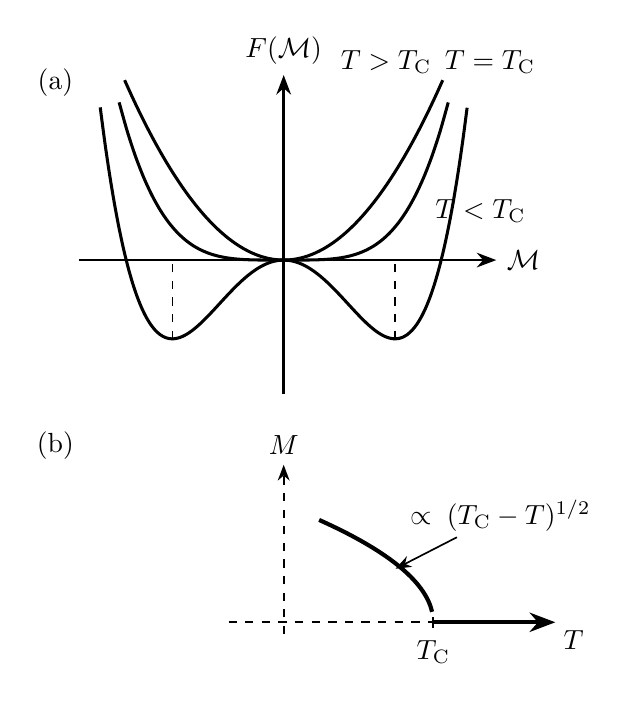
\begin{tikzpicture}[line width=0.8pt,>=Stealth]
% ================= (a) =================
\node at (-2.9,2.25) {(a)};
\draw[->,line width=0.9pt] (0,-1.7) -- (0,2.35) node[above] {$F(\mathcal{M})$};
\draw[->,line width=0.9pt] (-2.6,0) -- (2.7,0) node[right] {$\mathcal{M}$};
% T > T_C : steep single well
\draw[line width=1.1pt,domain=-2.02:2.02,samples=41,smooth]
  plot ({\x},{0.56*\x*\x});
% T = T_C : flat-bottom quartic
\draw[line width=1.1pt,domain=-2.09:2.09,samples=41,smooth]
  plot ({\x},{0.105*\x*\x*\x*\x});
% T < T_C : double well, minima at +/-1.414, F=-1
\draw[line width=1.1pt,domain=-2.33:2.33,samples=81,smooth]
  plot ({\x},{0.25*\x*\x*\x*\x-\x*\x});
\draw[dashed,line width=0.5pt] (1.414,-1) -- (1.414,0);
\draw[dashed,line width=0.5pt] (-1.414,-1) -- (-1.414,0);
\node at (1.3,2.52) {$T>T_{\mathrm{C}}$};
\node at (2.62,2.52) {$T=T_{\mathrm{C}}$};
\node at (2.5,0.62) {$T<T_{\mathrm{C}}$};
% ================= (b) =================
\begin{scope}[shift={(0,-4.6)}]
\node at (-2.9,2.25) {(b)};
% axes: vertical dashed with arrow (M), horizontal: thin dashed left of T_C then thick to arrow (T)
\draw[->,dashed,line width=0.6pt] (0,-0.15) -- (0,2.0) node[above] {$M$};
\draw[dashed,line width=0.6pt] (-0.7,0) -- (1.9,0);
\draw[->,line width=1.4pt] (1.9,0) -- (3.45,0) node[below right=-1pt] {$T$};
% M ~ (T_C - T)^{1/2} for T < T_C
\draw[line width=1.5pt,domain=0.45:1.885,samples=61,smooth]
  plot ({\x},{1.3*sqrt((1.9-\x)/1.45)});
% tick and label T_C
\draw[line width=0.8pt] (1.9,-0.07) -- (1.9,0.07);
\node at (1.9,-0.38) {$T_{\mathrm{C}}$};
% annotation with leader arrow
\node at (2.75,1.35) {$\propto\;(T_{\mathrm{C}}-T)^{1/2}$};
\draw[->,line width=0.6pt] (2.2,1.08) -- (1.42,0.68);
\end{scope}
\end{tikzpicture}
\end{document}
